\documentclass[a4paper, 12pt]{article}

\usepackage[T1]{fontenc}
\usepackage{booktabs}
\usepackage{IEEEtrantools}
\usepackage[]{amsmath}
\usepackage{amssymb}
\usepackage{float}
\usepackage[]{graphicx}
\usepackage{caption}
\usepackage{subcaption}

\title{Control Systems: Practical 4}
\author{216054484 216008466}

\begin{document}

\pagenumbering{gobble}
\maketitle
\newpage
\pagenumbering{roman}
\tableofcontents
\listoffigures
\newpage
\pagenumbering{arabic}

\section{Introduction} % (fold)
\label{sec:introduction}
The purpose of this practical is to model discrete controllers using approximation methods to convert a continuous controller to a digital controller  and a more accurate approach where a complete digital design of the plant and controller is done. Used in this practical is a lead compensator defined by the equation that follows
\begin{equation}
	\label{eq:lead_compensator}
	D_c(s) = 
\end{equation}

<+DISCUSSION OF THE PLANT+>

<+DISCUSSION OF CONTINUOUS CONTROL ON PLANT+>
\begin{figure}[H]
  \centering
  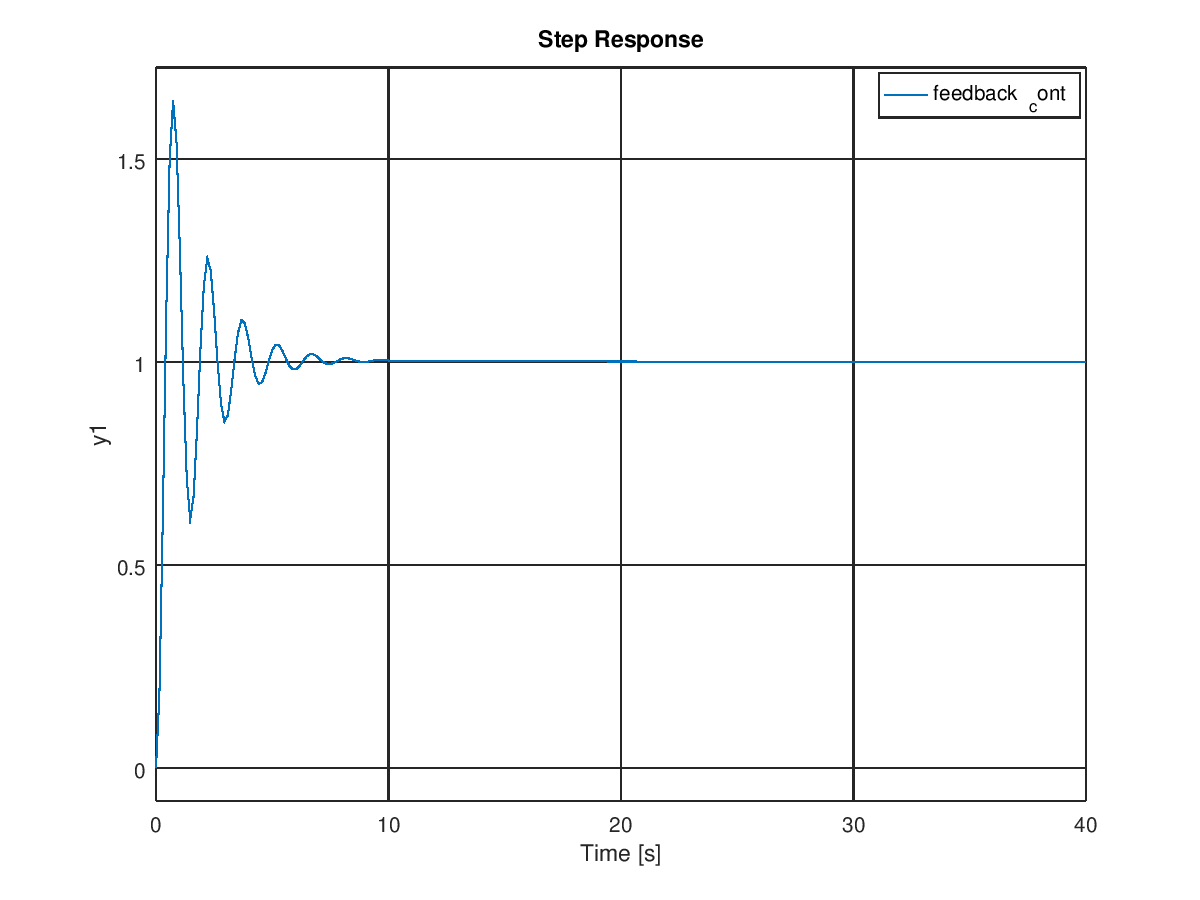
\includegraphics[width=\textwidth]{img/continuous_control.png}
  \caption{Continuous control using a lead compensator}
  \label{fig:continuous_control}
\end{figure}
% section introduction (end)

\section{Question 1} % (fold)
\label{sec:question_1}
The Tustin method of approximating the lead controller as defined by \eqref{eq:lead_compensator} was used to yield the discrete controller for the system in consideration. To follow are 4 different discrete controller results obtained for a number of different sampling times.

\begin{figure}[H]
  \centering
  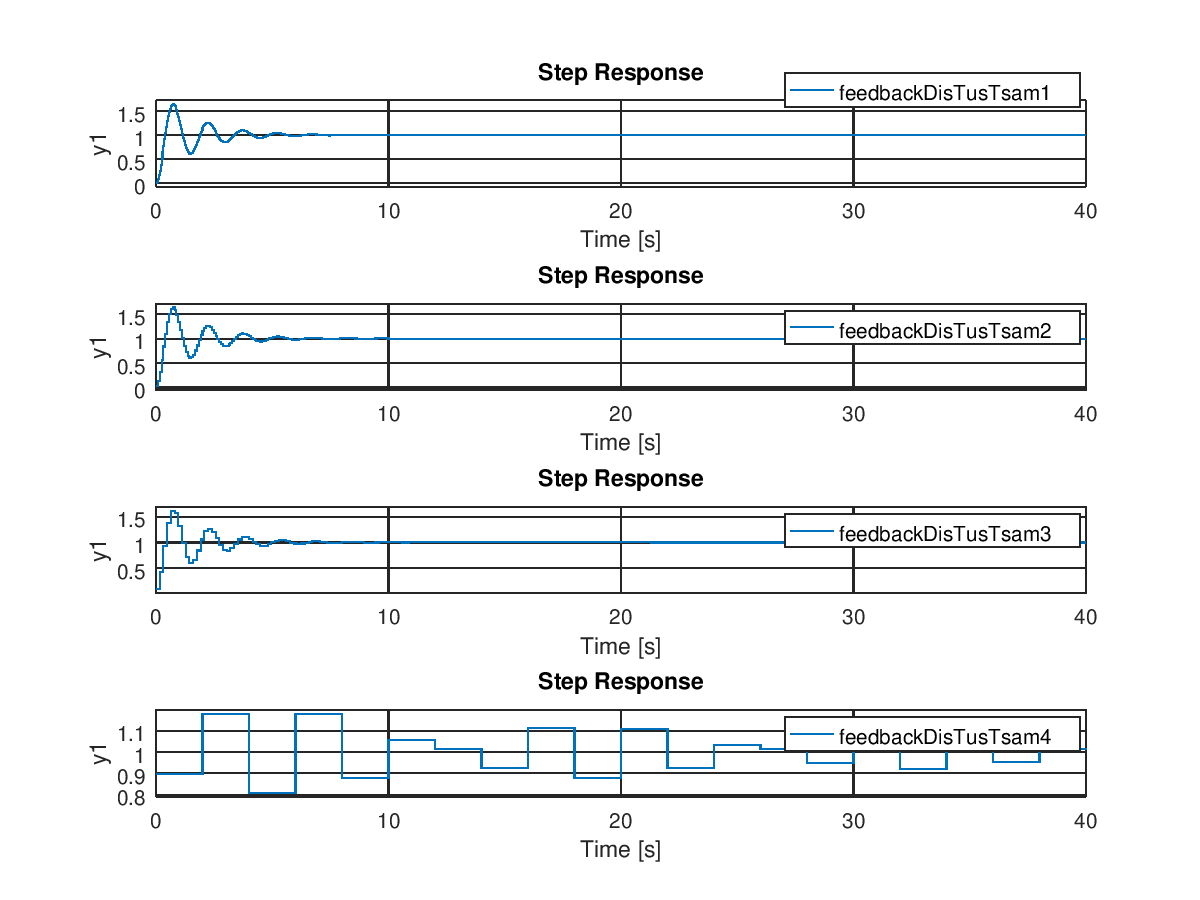
\includegraphics[width=\textwidth]{img/discrete_controllers.png}
  \caption{Discrete control of system using sample times of respectively 0.04, 0.08, 0.16 and 2 seconds}
  \label{fig:discrete_controllers}
\end{figure}

These plots were obtained by running the following octave code\\

  \noindent
  \texttt{plant = tf([5*9.8],[7 0 0]);}\\
  \texttt{plant\_dis\_tsam1 = c2d(plant,tsam1,'tustin');}\\
  \texttt{plant\_dis\_tsam2 = c2d(plant,tsam2,'tustin');}\\
  \texttt{plant\_dis\_tsam3 = c2d(plant,tsam3,'tustin');}\\
  \texttt{plant\_dis\_tsam4 = c2d(plant,tsam4,'tustin');}\\

  \noindent
  \texttt{cont\_cont = 0.28*tf([6.7 1],[0.106*6.7 1])}\\
  
  \noindent
  \texttt{feedback\_cont = feedback(plant*cont\_cont);}\\
  \texttt{figure;}\\
  \texttt{step(feedback\_cont)}\\
  
  \noindent
  \texttt{dis\_cont\_tus\_tsam1 = c2d(cont\_cont,tsam1,'tustin');}\\
  \texttt{dis\_cont\_tus\_tsam2 = c2d(cont\_cont,tsam2,'tustin');}\\
  \texttt{dis\_cont\_tus\_tsam3 = c2d(cont\_cont,tsam3,'tustin');}\\
  \texttt{dis\_cont\_tus\_tsam4 = c2d(cont\_cont,tsam4,'tustin');}\\
  
  \noindent
  \texttt{feedbackDisTusTsam1 = feedback(plant\_dis\_tsam1*dis\_cont\_tus\_tsam1);}\\
  \texttt{feedbackDisTusTsam2 = feedback(plant\_dis\_tsam2*dis\_cont\_tus\_tsam2);}\\
  \texttt{feedbackDisTusTsam3 = feedback(plant\_dis\_tsam3*dis\_cont\_tus\_tsam3);}\\
  \texttt{feedbackDisTusTsam4 = feedback(plant\_dis\_tsam4*dis\_cont\_tus\_tsam4);}\\
  
  \noindent
  \texttt{figure;}\\
  \texttt{subplot(4,1,1);}\\
  \texttt{step(feedbackDisTusTsam1)}\\
  \texttt{subplot(4,1,2);}\\
  \texttt{step(feedbackDisTusTsam2)}\\
  \texttt{subplot(4,1,3);}
  \texttt{step(feedbackDisTusTsam3)}\\
  \texttt{subplot(4,1,4);}\\
  \texttt{step(feedbackDisTusTsam4)}\\

The continuous system was made discrete in order to implement the feedback using the discrete controllers (another approach that would yield a better result is to use MATLAB's Simulink)\\

Now comparing these results with the application of the lead compensator, as dipicted in Figure \ref{fig:continuous_control}, we see that the best discrete approximation (that lies close to the step response of the continuously controlled system) is the Tustin discrete controller using a sampling time of $0.04$ seconds. As the sampling time increases (i.e. less samples are taken over the course of the same period) the approximation drifts off and the discrete controller doesn't provided the control that its continuous controller can provide (and should provide as the discrete controllers are approximations of the desired system response using a continuous controller).\\

The best sampling time yielding a close to exact replica of a system's response using a continuous controller is $20\times \omega_n$ where $\omega_n$ is the natural frequency of the system. Problems with the approximation come if the sampling time is chosen to be $10\times \omega_n$. It is safe to say that using a sampling time of $2$ seconds, is much less than $10\times \omega_n$ and sampling times of $0.04$, $0.08$ and $0.16$ lie closer to $20\times \omega_n$




% section question_1 (end)

\section{Question 2}

In this question we try to match the lead compensator's performance from the
previous question, at least in terms of rise-time. We attempt to do this using
the pole placement method. Noticing that our lead compensator exhibits quite a
bit of overshoot, we require the poles of our transfer function to be, first
and foremost, in the left hand half of the s-plane, but also that the poles
have an imaginary component, which yields the oscillatory motion as seen in
figure \ref{fig:continuous_control}.

By inspection, we find that pole locations of $p = -5 \pm j6$ give a good rise
time along with a good settling time. Sampling at $T = 0.06$ seconds, the step
input of our pole-placement system is given by figure \ref{fig:2_1}.

\begin{figure}[H]
	\centering
	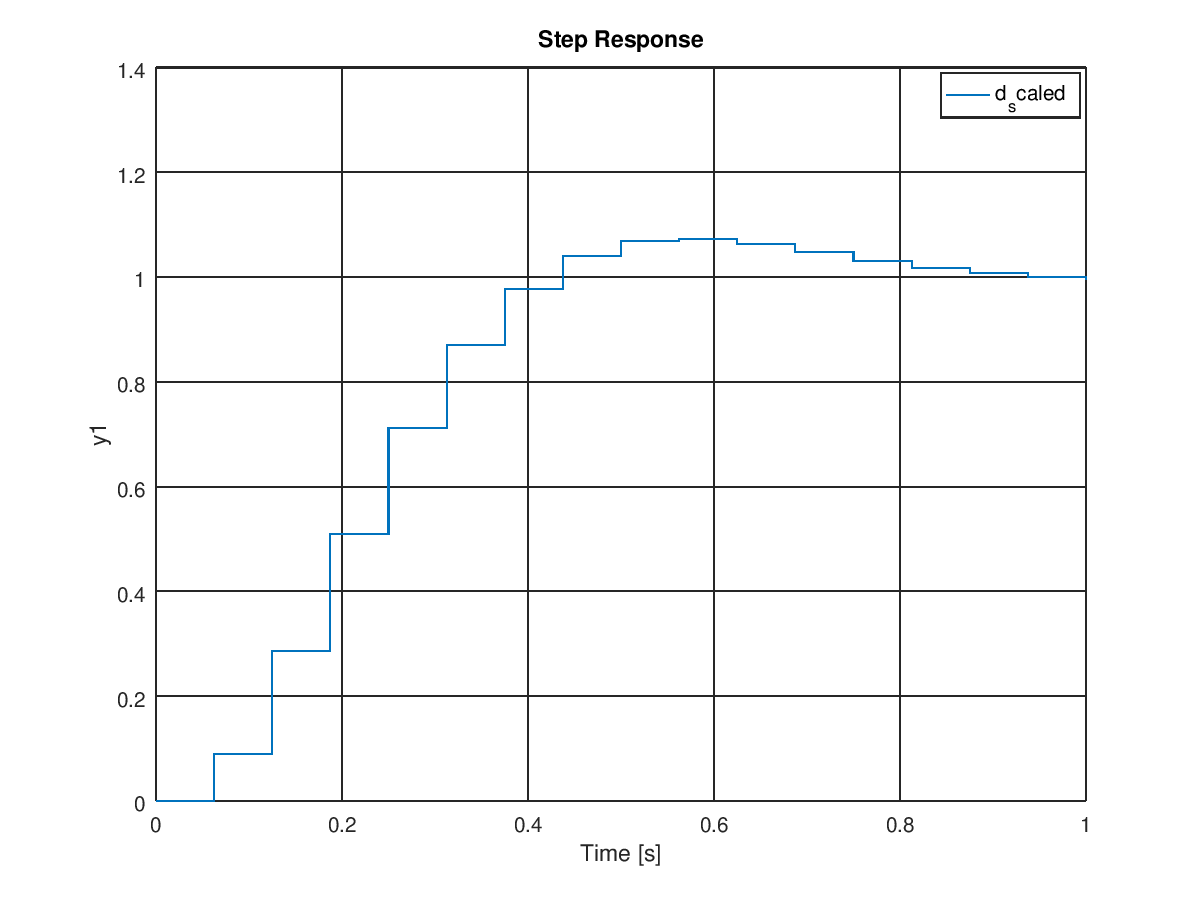
\includegraphics[width=\textwidth]{./img/2_1.png}
	\caption{ZOH system}
	\label{fig:2_1}
\end{figure}

This yields a rise-time of 0.25 seconds, which is very close to the original
rise time of 0.246 seconds. Furthermore, we can show how a reduced sampling
time negatively affects our system's performance in figure \ref{fig:2_2}. Not
only is there a large amount of aliasing taking place, the settling time is
also approximately 1.3 seconds, while the system from figure \ref{fig:2_1}
settles in about 1 second. Clearly, such a long sampling time is not adequate
to control the system.

\begin{figure}[H]
  \centering
  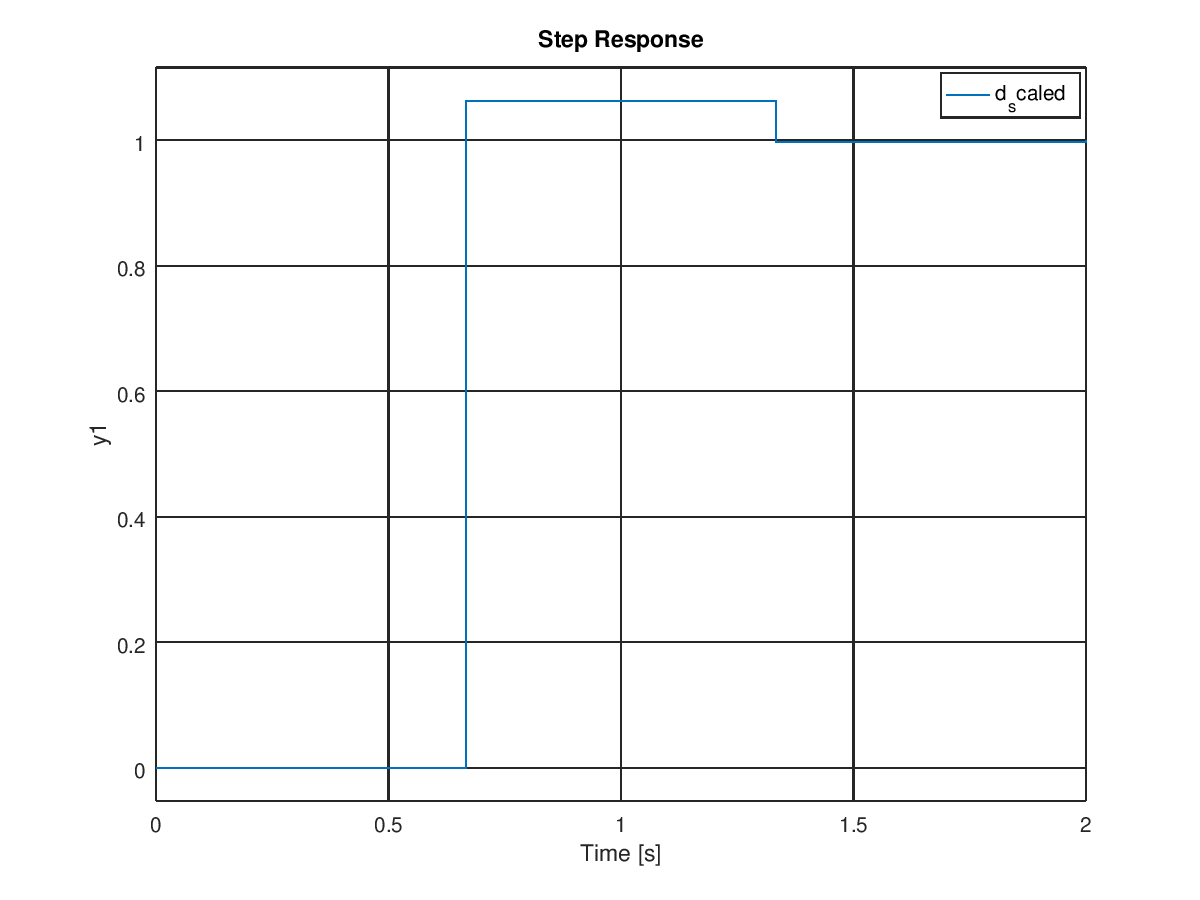
\includegraphics[width=\textwidth]{./img/2_2.png}
  \caption{ZOH system with T = 0.6 seconds}
  \label{fig:2_2}
\end{figure}

% section question_2 (end)

\section{Question 3}

Consider the general control system topology in Figure 8.28, question 2.4 of
the practical assignment. With consideration of the specifications of this
closed loop system, we find the following values that satisfy $\zeta > 0.5$ and
$\omega_n > 1$.

\begin{IEEEeqnarray}{lCl}
  K & = & 5 \label{eq:3_K}\\
  T_D & = & 0.6 \label{eq:3_td} \\
  T_I & = & 1.6667 \label{eq:3_ti}
\end{IEEEeqnarray}

Using the \texttt{damp()} function in Octave, we find that we have the
$\zeta$ and $\omega_n$ values for the system as given in table \ref{tab:specs}.

\begin{table}
  \centering
  \begin{tabular}{c c c}
    \toprule
    & $\zeta$ & $\omega_n$ \\
    \midrule
	$p_1$ & 0.69553 & 1.1031 \\
	$p_2$ & 0.69553 & 1.1031 \\
	$p_3$ & 1.00000 & 2.4656 \\
    \bottomrule
  \end{tabular}
  \caption{Damping ratio and natural frequency attributes of the system}
  \label{tab:specs}
\end{table}

Therefore we get the following negative feedback system, with the step input response given in figure

\begin{equation}
  G(s) = \frac{3 s^2 + 5s + 3}{s^3 + 4s^2 + 5s + 3}
  \label{eq:gs_original}
\end{equation}

\begin{figure}[H]
  \centering
  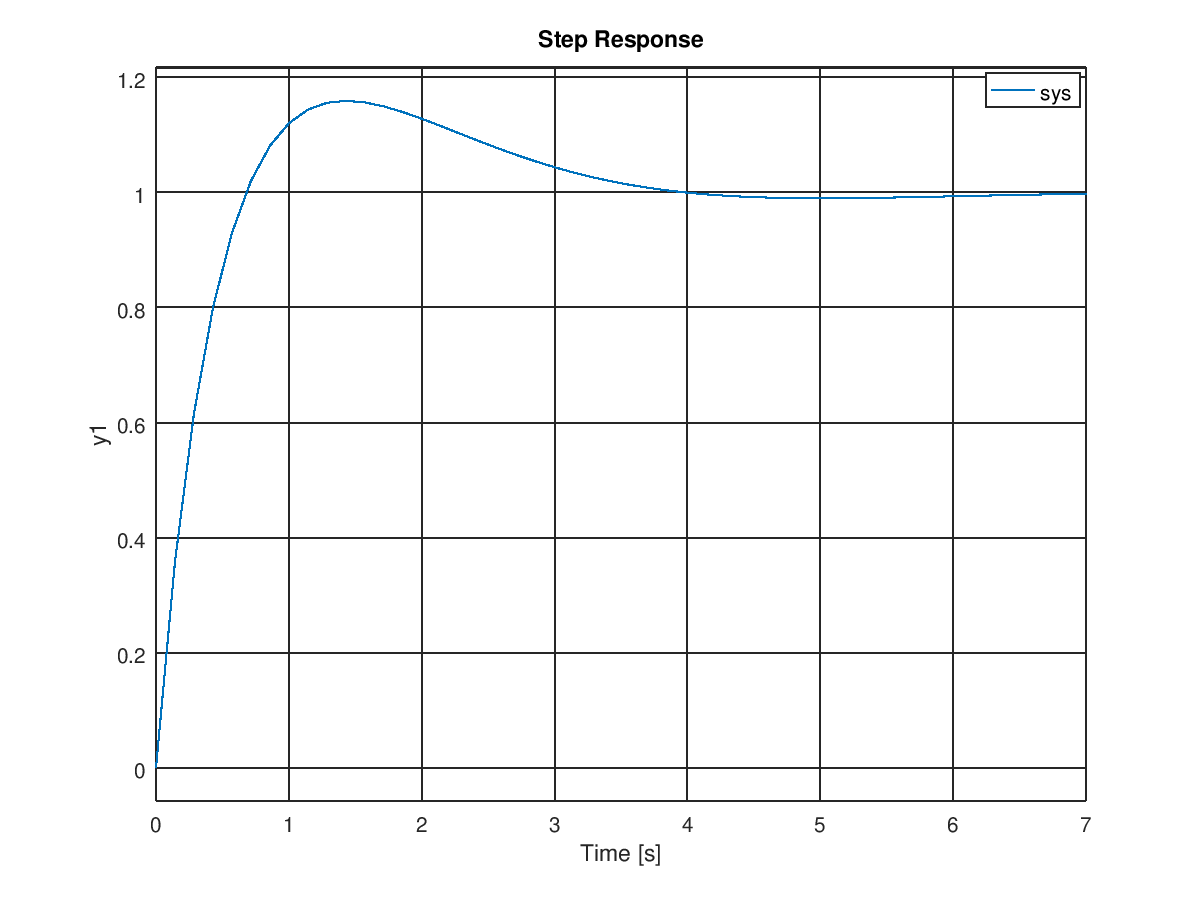
\includegraphics[width=.8\textwidth]{./img/2_5_continuous.png}
  \caption{Step input response of equation \eqref{eq:gs_original}}
  \label{fig:2_original}
\end{figure}

In the following sections, we present the different transfer functions and step
input responses for the discretized controllers based on \eqref{eq:gs_original}.

% tustin 1

\begin{equation}
  G_d(z) = \frac{0.6757 z^3 + 0.1892 z^2 - 0.3514 z + 0.1351}{z^3 - 0.5676 z^2 + 0.1892 z + 0.02703}
  \label{eq:tustin_1}
\end{equation}
% tustin .1
\begin{equation}
  G_d(z) = \frac{0.1343 z^3 - 0.1124 z^2 - 0.1331 z + 0.1137}{z^3 - 2.627 z^2 + 2.299 z - 0.6696}
  \label{eq:tustin_01}
\end{equation}
% tustin .01
\begin{equation}
  G_d(z) = \frac{0.01483 z^3 - 0.01458 z^2 - 0.01483 z + 0.01458}{z^3 - 2.96 z^2 + 2.921 z - 0.9608}
  \label{eq:tustin_001}
\end{equation}
% mpz 1
\begin{equation}
  G_d(z) = \frac{1.148 z^2 - 0.8495 z + 0.2169}{z^3 - 0.7369 z^2 + 0.271 z - 0.01832}
  \label{eq:mpz_1}
\end{equation}
% mpz .1
\begin{equation}
  G_d(z) = \frac{0.2675 z^2 - 0.4916 z + 0.2265}{z^3 - 2.628 z^2 + 2.301 z - 0.6703}
  \label{eq_mpz_01}
\end{equation}
% mpz .01
\begin{equation}
  G_d(z) = \frac{0.02965 z^2 - 0.05881 z + 0.02916}{z^3 - 2.96 z^2 + 2.921 z - 0.9608}
  \label{eq:mpz_001}
\end{equation}

To enhance the discussion, the graphs of the step responses have been provided.
As we can see in figure \ref{fig:tustin001} and figure \ref{fig:mpz001},
sampling at a very quick rate of 0.01 seconds, we can see that the discrete
system matches the continuous version almost exactly, with no real appreciable
difference. Looking at figures \ref{fig:tustin01} and \ref{fig:mpz01}, we can
now clearly see the reduced resolution by sampling at 0.1 second intervals.
However, the general characteristics seem to have been preserved in the system.
The overshoot, rise times, and settling times for both methods seems to have
been preserved. Looking at figure \ref{fig:tustin1} and figure \ref{fig:mpz1}
though, we see that a sampling rate of 1 second seems to drastically affect the
discrete system. The overshoot is drastically increased to more than 25\% for
the Tustin method.

\begin{figure}[H]
  \centering
  \begin{subfigure}{.6\textwidth}
    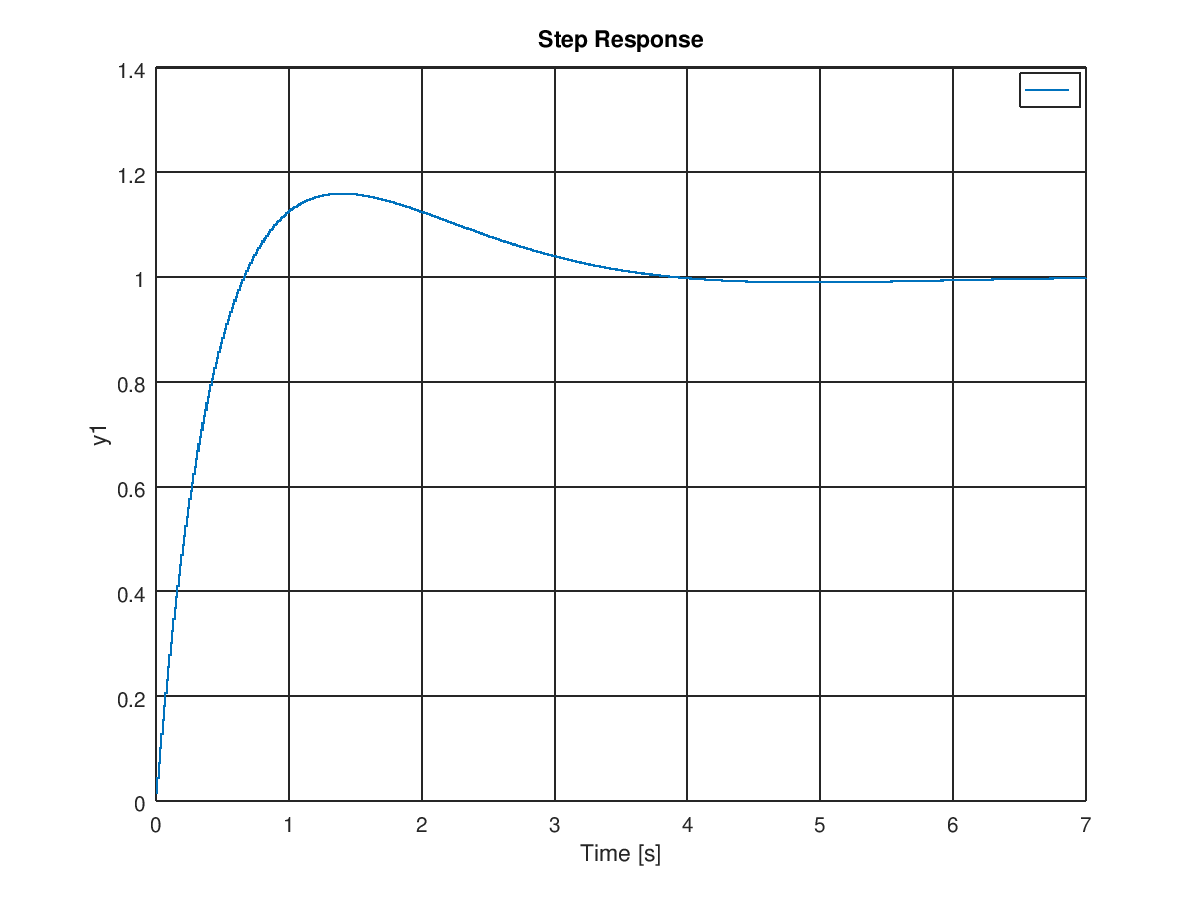
\includegraphics[width=\textwidth]{./img/2_5_tustin001.png}
    \caption{$T = 0.01$ seconds}
    \label{fig:tustin001}
  \end{subfigure}

  \begin{subfigure}{.6\textwidth}
    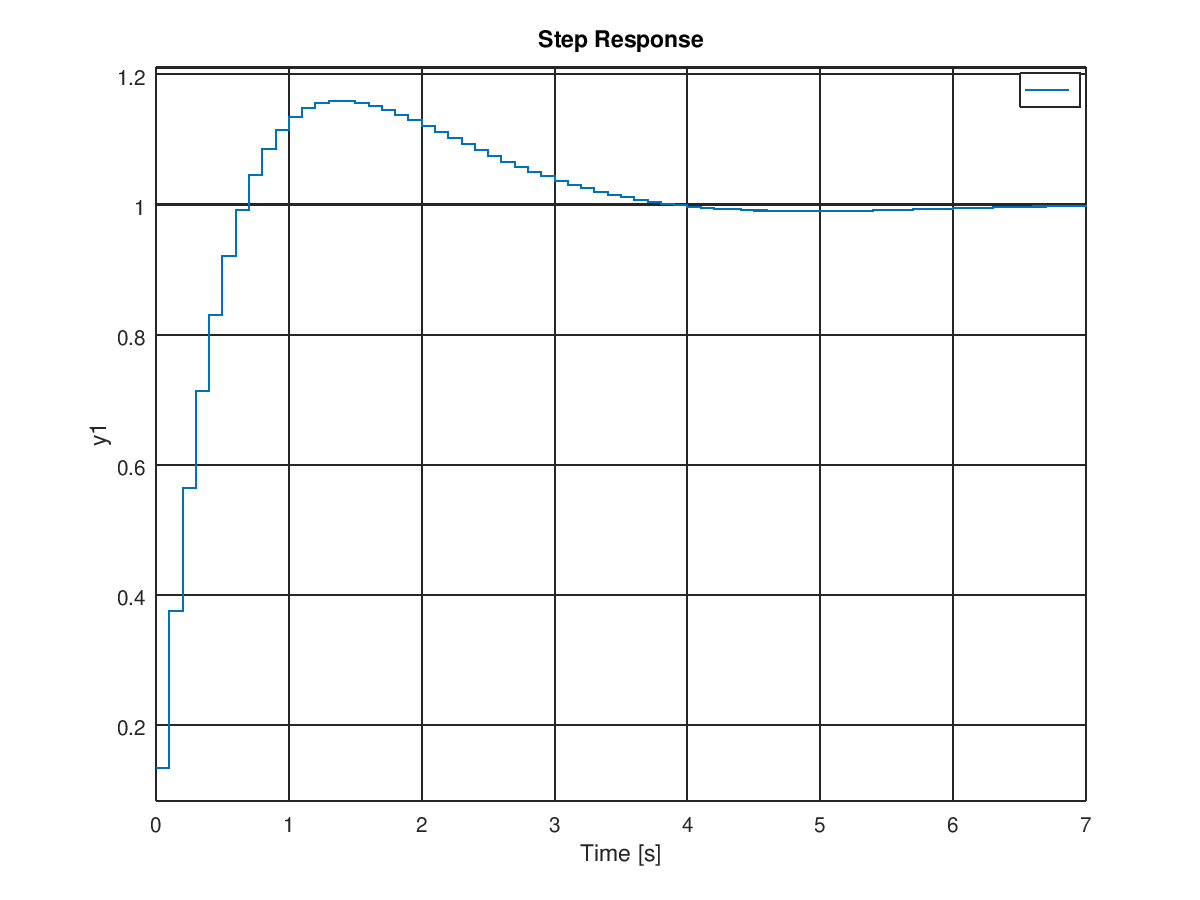
\includegraphics[width=\textwidth]{./img/2_5_tustin01.png}
    \caption{$T = 0.1$ seconds}
    \label{fig:tustin01}
  \end{subfigure}
  
  \begin{subfigure}{.6\textwidth}
    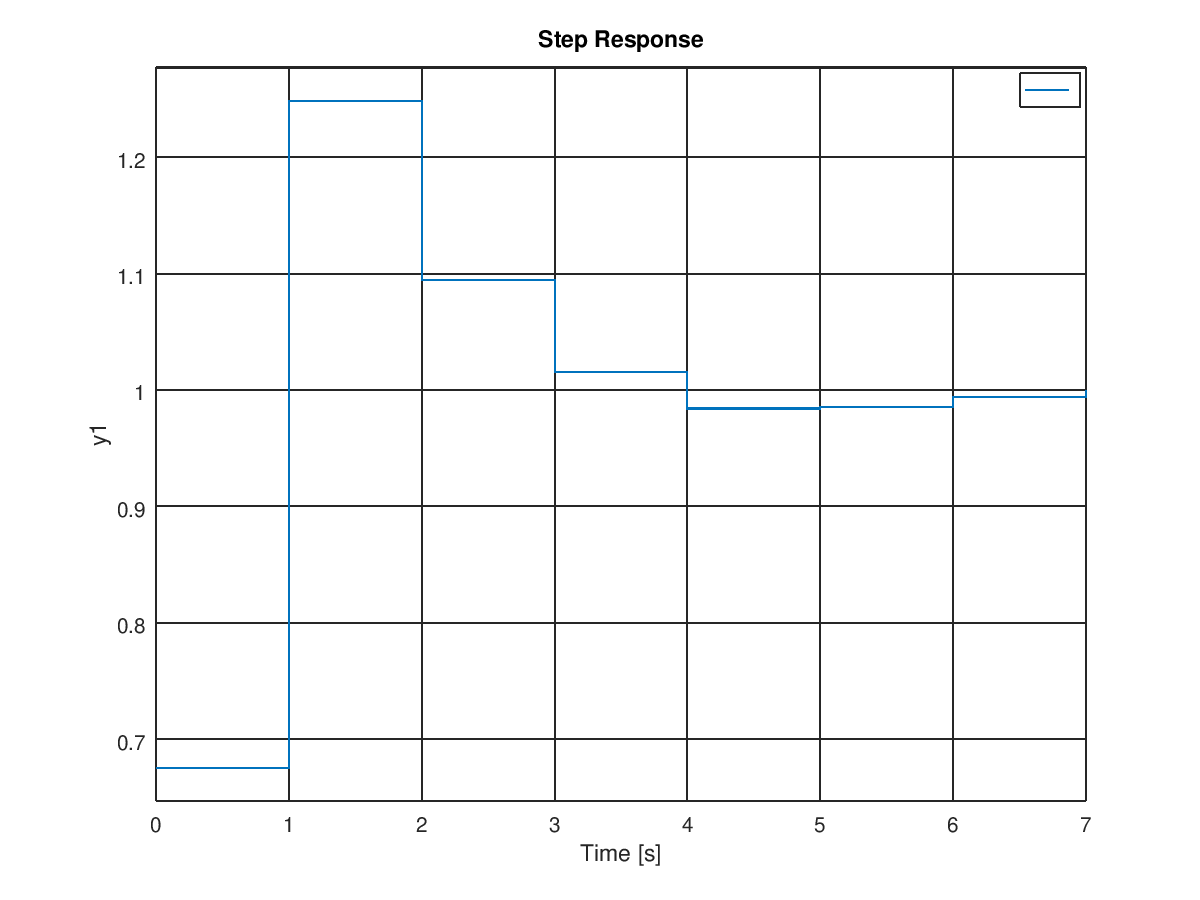
\includegraphics[width=\textwidth]{./img/2_5_tustin1.png}
    \caption{$T = 1$ second}
    \label{fig:tustin1}
  \end{subfigure}
  \caption{Tustin emulation}
\end{figure}

\begin{figure}[H]
  \centering
  \begin{subfigure}{.6\textwidth}
    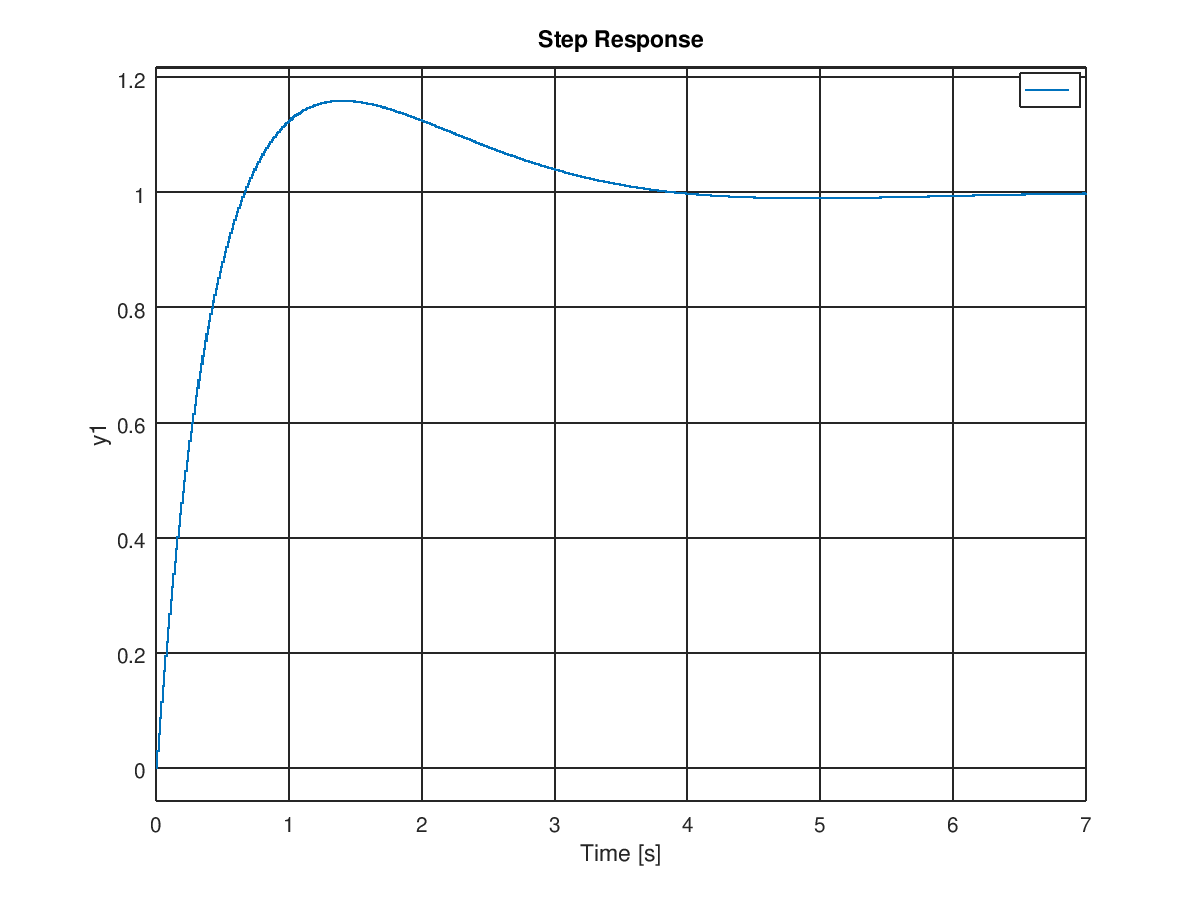
\includegraphics[width=\textwidth]{./img/2_5_mpz001.png}
    \caption{$T = 0.01$ seconds}
    \label{fig:mpz001}
  \end{subfigure}

  \begin{subfigure}{.6\textwidth}
    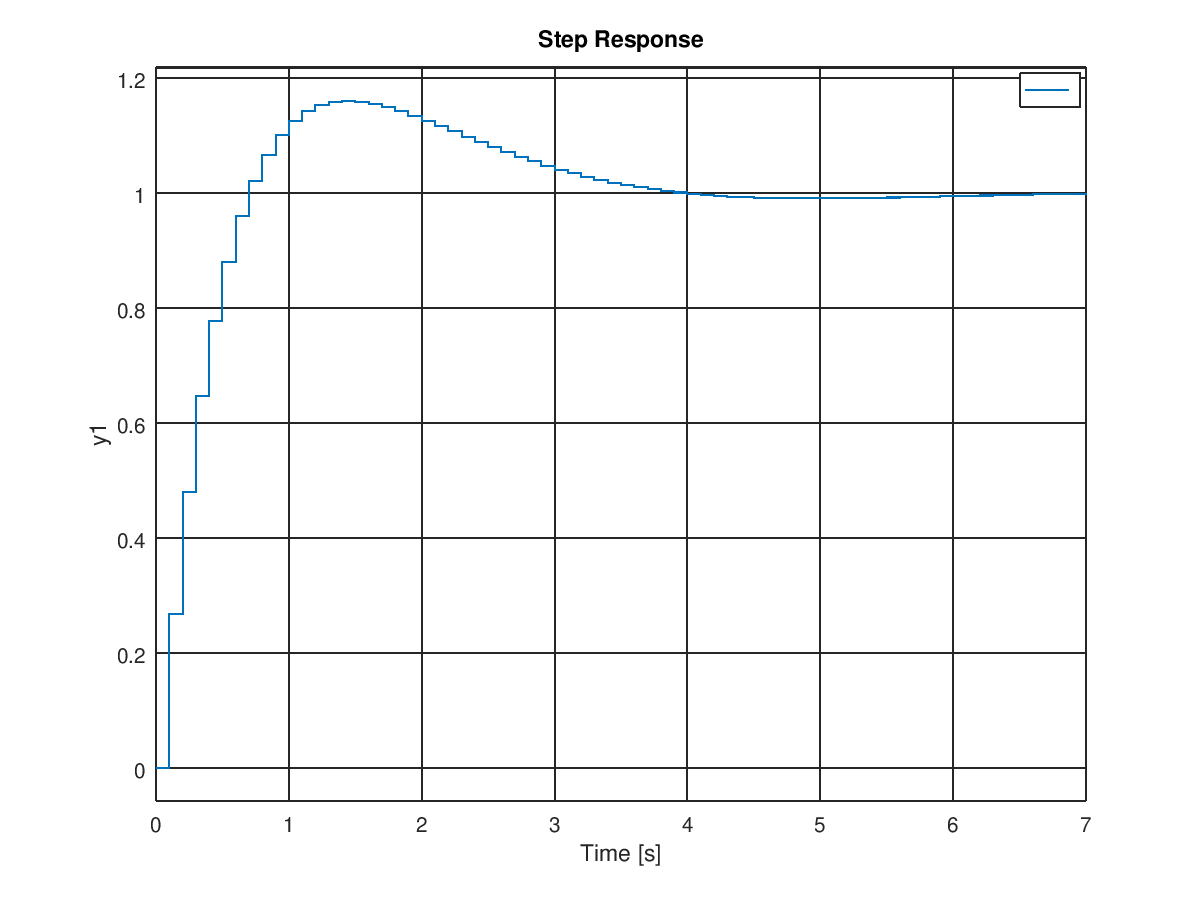
\includegraphics[width=\textwidth]{./img/2_5_mpz01.png}
    \caption{$T = 0.1$ seconds}
    \label{fig:mpz01}
  \end{subfigure}
  
  \begin{subfigure}{.6\textwidth}
    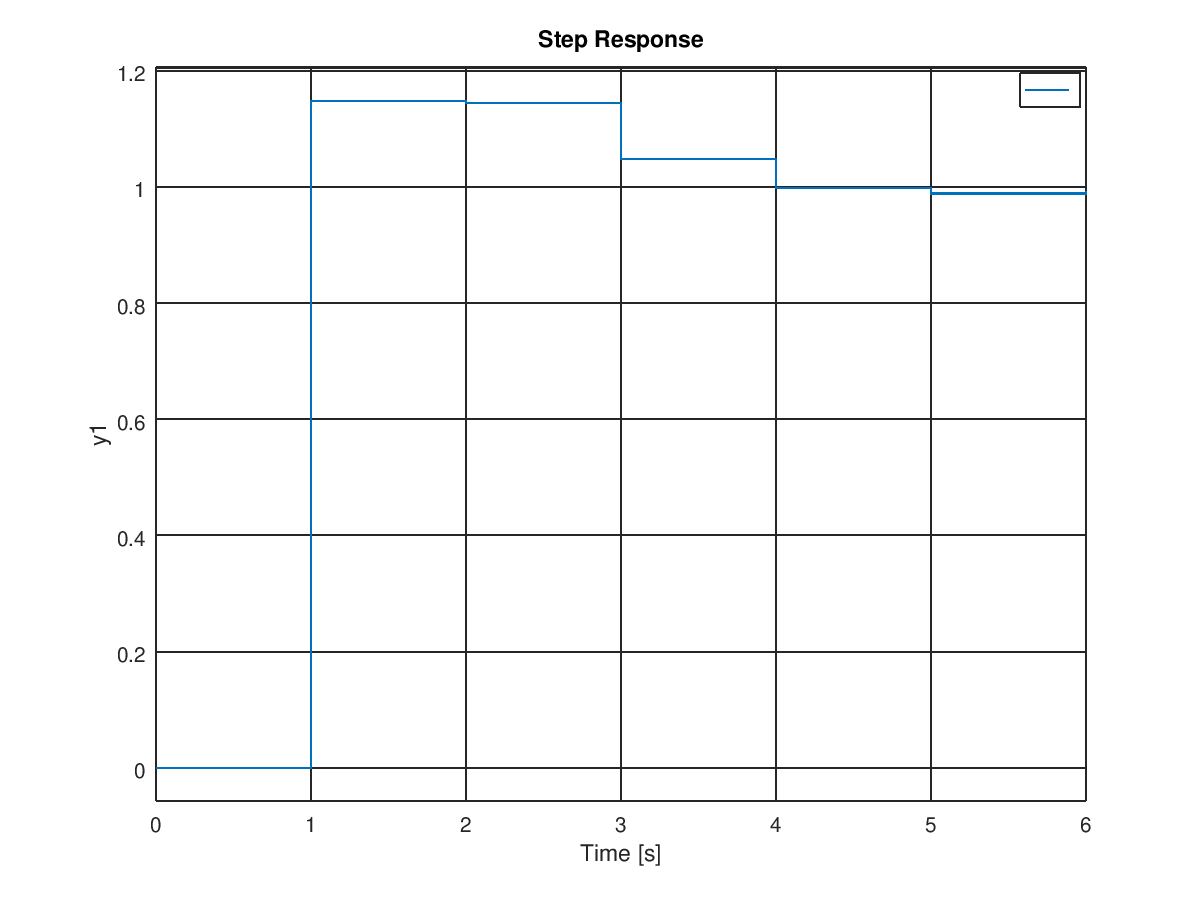
\includegraphics[width=\textwidth]{./img/2_5_mpz1.png}
    \caption{$T = 1$ second}
    \label{fig:mpz1}
  \end{subfigure}
  \caption{Matched Pole-Zero emulation}
\end{figure}
% section question_3 (end)
\end{document}
